\appendix

\chapter{AES körlägestest resultat}
\label{app:raw-data-mode-picture-test}

\section{Före testet}
\begin{figure}[H]
  \centering
  
\includegraphics[width=0.6\textwidth]{pi.png}
  \caption{Orginal bild}
  \label{fig:pi-original}
\end{figure}

\section{Efter ECB kryptering}
\begin{figure}[H]
  \centering
  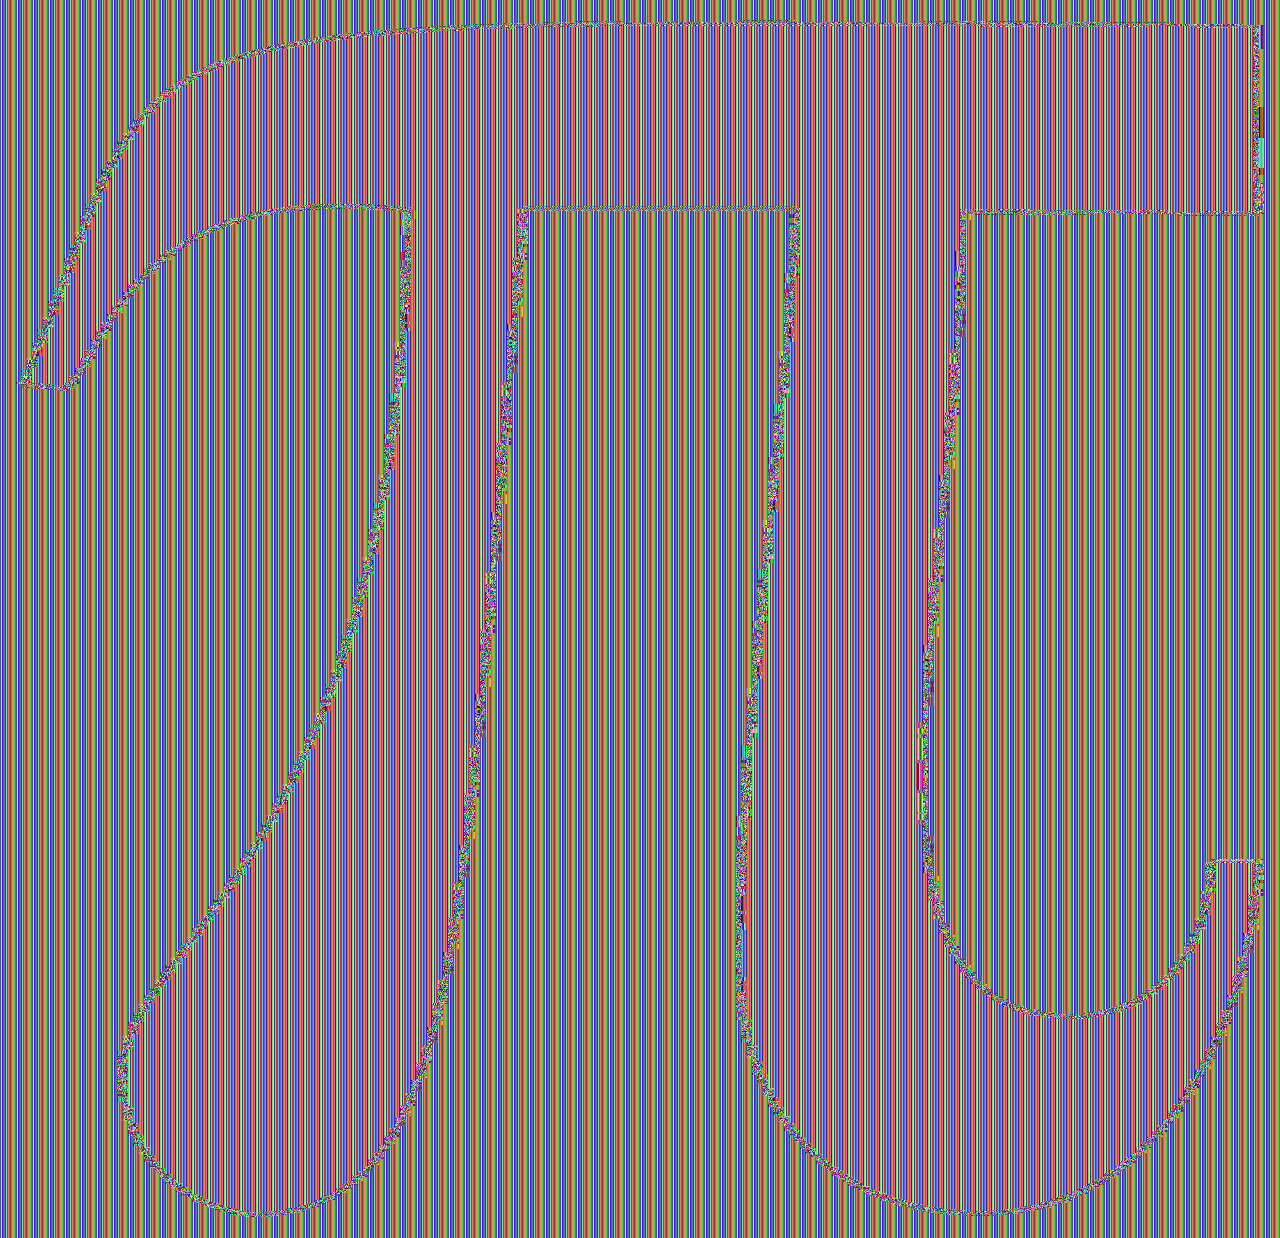
\includegraphics[width=0.6\textwidth]{pi-ecb.png}
  \caption{Efter ECB Kryptering}
  \label{fig:pi-ecb}
\end{figure}

\section{Efter CBC kryptering}
\begin{figure}[H]
  \centering
  \includegraphics[width=0.6\textwidth]{pi-cbc.png}
  \caption{Efter CBC Kryptering}
  \label{fig:pi-cbc}
\end{figure}

\section{Efter CFB kryptering}
\begin{figure}[H]
  \centering
  \includegraphics[width=0.6\textwidth]{pi-OFB.png}
  \caption{Efter OFB Kryptering}
  \label{fig:pi-ofb}
\end{figure}

\cleardoublepage

\chapter{Fullständig data från testerna}
\label{app:raw-data}

\section{Data från nyckellängdstest}
\label{app:raw-data-keylength}

\begin{table}[H]
    \centering
    \begin{tabular}{ ||c|c|c|| }
      \hline
      \multicolumn{3}{|c|}{\bfseries{Resultat Tid (s)}} \\
      \hline
      \bfseries{ECB - 128bit} & \bfseries{ECB - 192bit} & \bfseries{ECB - 256bit} \\
      \hline
      21.114332500001183 & 25.019810000005236 & 29.25573820000136 \\
      21.2294222000055 & 25.03902250000101 & 29.199436000002606 \\
      21.400101300001552 & 24.921688300004462 & 29.1446350000042 \\
      21.394803399998636 & 25.010479399999895 & 29.276371100000688 \\
      21.410092899997835 & 25.023025200003758 & 29.208361999997578 \\
      21.255479499996 & 24.94711079999979 & 29.12308629999461 \\
      21.709606899996288 & 24.932161500000802 & 29.057567500000005 \\
      20.930029600000125 & 24.93615460000001 & 29.23549970000022 \\
      20.91164679999929 & 25.07268920000206 & 29.163480200004415 \\
      21.024735999999393 & 25.05104990000109 & 29.13999270000204 \\
      20.974247600002855 & 24.92792770000233 & 29.03159289999894 \\
      20.906690399999206 & 25.040346800000407 & 29.238432199999806 \\
      20.949946799999452 & 25.02671339999506 & 29.226332500002172 \\
      20.96879309999349 & 24.999294099994586 & 29.13317239999742 \\
      20.955687699999544 & 24.973698000001605 & 29.119369399995776 \\
      20.907472200000484 & 24.992430599995714 & 29.273320899999817 \\
      20.99763510000048 & 25.22444600000017 & 29.147454799996922 \\
      20.964201399998274 & 25.310352100001182 & 29.133893199999875 \\
      20.970198600000003 & 25.03863189999538 & 29.14858010000171 \\
      21.033452000003308 & 24.887886799995613 & 29.20511969999643 \\
      20.835713899999973 & 25.002411200002825 & 29.214967400002934 \\
      20.933525599997665 & 25.029954099998577 & 29.155635700000857 \\
      20.899700900001335 & 24.92795739999565 & 29.136839000006148 \\
      20.861958300003607 & 25.015061800004332 & 29.250083099999756 \\
      20.898621000000276 & 25.012236000002304 & 29.22063089999574 \\
      \hline
    \end{tabular}
  \end{table}

\section{Data från körlägestest}
\label{app:raw-data-mode}

\begin{table}[H]
    \centering
    \begin{tabular}{ ||c|c|c|| }
      \hline
      \multicolumn{3}{|c|}{\bfseries{Resultat Tid (s)}} \\
      \hline
      \bfseries{ECB} & \bfseries{CBC} & \bfseries{OFB} \\
      \hline
      20.855055499996524 & 20.863876399998844 & 20.801168300000427 \\
      20.88846609999746 & 20.907602499995846 & 20.78754040000058 \\
      20.879108299996005 & 20.86540999999852 & 20.823867599996447 \\
      20.801008999995247 & 20.896374500000093 & 20.87718119999772 \\
      20.85887470000307 & 20.868871400001808 & 20.770114799997828 \\
      20.87116899999819 & 20.882914800000435 & 20.767576799997187 \\
      20.854077200005122 & 20.89511720000155 & 20.85902029999852 \\
      20.85488130000158 & 20.85610540000198 & 20.797623000005842 \\
      20.826587200004724 & 20.865844100000686 & 20.796596600004705 \\
      20.909639099998458 & 20.85497480000049 & 20.797125700002653 \\
      20.870294899999863 & 20.906652400000894 & 20.835499799999525 \\
      20.818692400003783 & 20.92016809999768 & 20.865253799995116 \\
      20.82849349999742 & 20.908798900003603 & 20.800847200000135 \\
      20.86879109999427 & 20.850567699999374 & 20.795617399999173 \\
      20.91046159999678 & 20.883563499999582 & 20.834485100000165 \\
      20.82723100000294 & 20.884897599993565 & 20.82335030000104 \\
      20.80391700000473 & 20.89037549999921 & 20.828929399998742 \\
      20.87521669999842 & 20.885131600000022 & 20.811529400001746 \\
      20.91481080000085 & 20.93468269999721 & 20.881663000000117 \\
      21.085760299996764 & 20.859826599997177 & 20.85081160000118 \\
      20.97296980000101 & 20.875606900001003 & 20.823041400006332 \\
      21.053496200001973 & 20.903108300000895 & 20.791531299997587 \\
      20.978821899996547 & 20.892179500006023 & 20.878361099996255 \\
      20.954259099999035 & 20.890548900002614 & 20.873186500000884 \\
      21.028453000006266 & 20.88354160000017 & 20.76938550000341 \\
      \hline
    \end{tabular}
  \end{table}

\chapter{AES Implementering i python}
\label{app:python}

\section{AES.py}

\begin{python}
# ---------------
# Imported libraries
# ---------------
from os.path import getsize
from os import remove
import numpy as np

# ---------------
# Fixed variables
# ---------------
# Sbox & inverse Sbox
subBytesTable = (
    0x63, 0x7c, 0x77, 0x7b, 0xf2, 0x6b, 0x6f, 0xc5, 0x30, 0x01, 0x67, 0x2b, 0xfe, 0xd7, 0xab, 0x76,
    0xca, 0x82, 0xc9, 0x7d, 0xfa, 0x59, 0x47, 0xf0, 0xad, 0xd4, 0xa2, 0xaf, 0x9c, 0xa4, 0x72, 0xc0,
    0xb7, 0xfd, 0x93, 0x26, 0x36, 0x3f, 0xf7, 0xcc, 0x34, 0xa5, 0xe5, 0xf1, 0x71, 0xd8, 0x31, 0x15,
    0x04, 0xc7, 0x23, 0xc3, 0x18, 0x96, 0x05, 0x9a, 0x07, 0x12, 0x80, 0xe2, 0xeb, 0x27, 0xb2, 0x75,
    0x09, 0x83, 0x2c, 0x1a, 0x1b, 0x6e, 0x5a, 0xa0, 0x52, 0x3b, 0xd6, 0xb3, 0x29, 0xe3, 0x2f, 0x84,
    0x53, 0xd1, 0x00, 0xed, 0x20, 0xfc, 0xb1, 0x5b, 0x6a, 0xcb, 0xbe, 0x39, 0x4a, 0x4c, 0x58, 0xcf,
    0xd0, 0xef, 0xaa, 0xfb, 0x43, 0x4d, 0x33, 0x85, 0x45, 0xf9, 0x02, 0x7f, 0x50, 0x3c, 0x9f, 0xa8,
    0x51, 0xa3, 0x40, 0x8f, 0x92, 0x9d, 0x38, 0xf5, 0xbc, 0xb6, 0xda, 0x21, 0x10, 0xff, 0xf3, 0xd2,
    0xcd, 0x0c, 0x13, 0xec, 0x5f, 0x97, 0x44, 0x17, 0xc4, 0xa7, 0x7e, 0x3d, 0x64, 0x5d, 0x19, 0x73,
    0x60, 0x81, 0x4f, 0xdc, 0x22, 0x2a, 0x90, 0x88, 0x46, 0xee, 0xb8, 0x14, 0xde, 0x5e, 0x0b, 0xdb,
    0xe0, 0x32, 0x3a, 0x0a, 0x49, 0x06, 0x24, 0x5c, 0xc2, 0xd3, 0xac, 0x62, 0x91, 0x95, 0xe4, 0x79,
    0xe7, 0xc8, 0x37, 0x6d, 0x8d, 0xd5, 0x4e, 0xa9, 0x6c, 0x56, 0xf4, 0xea, 0x65, 0x7a, 0xae, 0x08,
    0xba, 0x78, 0x25, 0x2e, 0x1c, 0xa6, 0xb4, 0xc6, 0xe8, 0xdd, 0x74, 0x1f, 0x4b, 0xbd, 0x8b, 0x8a,
    0x70, 0x3e, 0xb5, 0x66, 0x48, 0x03, 0xf6, 0x0e, 0x61, 0x35, 0x57, 0xb9, 0x86, 0xc1, 0x1d, 0x9e,
    0xe1, 0xf8, 0x98, 0x11, 0x69, 0xd9, 0x8e, 0x94, 0x9b, 0x1e, 0x87, 0xe9, 0xce, 0x55, 0x28, 0xdf,
    0x8c, 0xa1, 0x89, 0x0d, 0xbf, 0xe6, 0x42, 0x68, 0x41, 0x99, 0x2d, 0x0f, 0xb0, 0x54, 0xbb, 0x16
    )

invSubBytesTable = (
    0x52, 0x09,	0x6a, 0xd5, 0x30, 0x36,	0xa5, 0x38,	0xbf, 0x40,	0xa3, 0x9e, 0x81, 0xf3, 0xd7, 0xfb,
    0x7c, 0xe3,	0x39, 0x82, 0x9b, 0x2f,	0xff, 0x87,	0x34, 0x8e,	0x43, 0x44, 0xc4, 0xde, 0xe9, 0xcb,
    0x54, 0x7b,	0x94, 0x32, 0xa6, 0xc2,	0x23, 0x3d,	0xee, 0x4c,	0x95, 0x0b, 0x42, 0xfa, 0xc3, 0x4e,
    0x08, 0x2e,	0xa1, 0x66, 0x28, 0xd9,	0x24, 0xb2,	0x76, 0x5b,	0xa2, 0x49, 0x6d, 0x8b, 0xd1, 0x25,
    0x72, 0xf8,	0xf6, 0x64, 0x86, 0x68,	0x98, 0x16,	0xd4, 0xa4,	0x5c, 0xcc, 0x5d, 0x65, 0xb6, 0x92,
    0x6c, 0x70,	0x48, 0x50, 0xfd, 0xed,	0xb9, 0xda,	0x5e, 0x15,	0x46, 0x57, 0xa7, 0x8d, 0x9d, 0x84,
    0x90, 0xd8,	0xab, 0x00, 0x8c, 0xbc,	0xd3, 0x0a,	0xf7, 0xe4,	0x58, 0x05, 0xb8, 0xb3, 0x45, 0x06,
    0xd0, 0x2c,	0x1e, 0x8f, 0xca, 0x3f,	0x0f, 0x02,	0xc1, 0xaf,	0xbd, 0x03, 0x01, 0x13, 0x8a, 0x6b,
    0x3a, 0x91,	0x11, 0x41, 0x4f, 0x67,	0xdc, 0xea,	0x97, 0xf2,	0xcf, 0xce, 0xf0, 0xb4, 0xe6, 0x73,
    0x96, 0xac,	0x74, 0x22, 0xe7, 0xad,	0x35, 0x85,	0xe2, 0xf9,	0x37, 0xe8, 0x1c, 0x75, 0xdf, 0x6e,
    0x47, 0xf1,	0x1a, 0x71, 0x1d, 0x29,	0xc5, 0x89,	0x6f, 0xb7,	0x62, 0x0e, 0xaa, 0x18, 0xbe, 0x1b,
    0xfc, 0x56,	0x3e, 0x4b, 0xc6, 0xd2,	0x79, 0x20,	0x9a, 0xdb,	0xc0, 0xfe, 0x78, 0xcd, 0x5a, 0xf4,
    0x1f, 0xdd,	0xa8, 0x33, 0x88, 0x07,	0xc7, 0x31,	0xb1, 0x12,	0x10, 0x59, 0x27, 0x80, 0xec, 0x5f,
    0x60, 0x51,	0x7f, 0xa9, 0x19, 0xb5,	0x4a, 0x0d,	0x2d, 0xe5,	0x7a, 0x9f, 0x93, 0xc9, 0x9c, 0xef,
    0xa0, 0xe0,	0x3b, 0x4d, 0xae, 0x2a,	0xf5, 0xb0,	0xc8, 0xeb,	0xbb, 0x3c, 0x83, 0x53, 0x99, 0x61,
    0x17, 0x2b,	0x04, 0x7e, 0xba, 0x77,	0xd6, 0x26,	0xe1, 0x69,	0x14, 0x63, 0x55, 0x21, 0x0c, 0x7d
    )

# Round constants
round_constant = (
    0x00000000, 0x01000000, 0x02000000,
    0x04000000, 0x08000000, 0x10000000,
    0x20000000, 0x40000000, 0x80000000,
    0x1B000000, 0x36000000, 0x6C000000,
    0xD8000000, 0xAB000000, 0x4D000000,
    )


# ---------------
# Main action functions
# ---------------
# Xtime
# Used to preform multiplication by x in the Galois field
def xtime(a):
    return (((a << 1) ^ 0x1B) & 0xFF) if (a & 0x80) else (a << 1)


# Byte substitution function
# Substitutes each byte in the state with a byte from the S-Box
def sub_bytes(data, bytesTable):
    for i, row in enumerate(data):
        for j, byte in enumerate(row):
            data[i][j] = bytesTable[byte]
    return data


# Shift rows function
# Shifts the rows of the the matrix to the left.
# Each row is shifted by the number of its index
def shift_rows(array):
    array[:, 1] = np.roll(array[:, 1], -1, axis=0)
    array[:, 2] = np.roll(array[:, 2], -2, axis=0)
    array[:, 3] = np.roll(array[:, 3], -3, axis=0)
    return array


# Inverse shift rows function
# Shifts the rows of the the matrix to the right.
# Each row is shifted by the number of its index
def inv_shift_rows(array):
    array[:, 1] = np.roll(array[:, 1], 1, axis=0)
    array[:, 2] = np.roll(array[:, 2], 2, axis=0)
    array[:, 3] = np.roll(array[:, 3], 3, axis=0)
    return array


# Performs the mix columns layer
def mix_columns(data):
    # mixes a single column
    def mix_single_column(data):
        t = data[0] ^ data[1] ^ data[2] ^ data[3]
        u = data[0]
        data[0] ^= t ^ xtime(data[0] ^ data[1])
        data[1] ^= t ^ xtime(data[1] ^ data[2])
        data[2] ^= t ^ xtime(data[2] ^ data[3])
        data[3] ^= t ^ xtime(data[3] ^ u)

    # mixes all columns using mix_single_column
    def mix(data):
        for i in range(4):
            mix_single_column(data[i])
        return data
    data = mix(data)
    return data


# Preforms the inverse mix columns layer
# This function is similar to the mix_columns function
# but instead preforms the inverse operation.
def inv_mix_columns(data):
    for i in range(4):
        u = xtime(xtime(data[i][0] ^ data[i][2]))
        v = xtime(xtime(data[i][1] ^ data[i][3]))
        data[i][0] ^= u
        data[i][1] ^= v
        data[i][2] ^= u
        data[i][3] ^= v
    mix_columns(data)
    return data


# Adds a padding to ensure a bloke size of 16 bytes
def add_padding(data):
    length = 16 - len(data)
    for i in range(length):
        data.append(0)
    return data, length


# Removes the padding from the data
def remove_padding(data, identifier):
    if identifier[-1] == 0:
        return data
    elif identifier[-1] > 0 and identifier[-1] < 16:
        return data[:-identifier[-1]]
    else:
        raise ValueError('Invalid padding')


# Performs the encryption rounds on the input data matrix
# This function is used for the encryption of data matrixes
# using the expanded keys.
def encryption_rounds(data, round_keys, nr):
    # Inizial add round key
    data = np.bitwise_xor(data, round_keys[0])

    # Rounds 1 to 9 or 1 to 11 or 1 to 13
    # Here each step in one round is performed in a sequence n times
    # where n is the number of rounds minus the last round.
    for i in range(1, (nr - 1)):
        # Sub bytes
        data = sub_bytes(data, subBytesTable)
        # Shift rows
        data = shift_rows(data)
        # Mix columns
        data = mix_columns(data)
        # Add round key
        data = np.bitwise_xor(data, round_keys[i])

    # Final round
    # Identical to the previous rounds, but without mix columns
    data = sub_bytes(data, subBytesTable)
    data = shift_rows(data)
    data = np.bitwise_xor(data, round_keys[nr - 1])

    # Returns the encrypted data
    return data


# Performs the decryption rounds on the input data matrix
# This function is used for the decryption of data matrixes
# using the expanded keys.
def decryption_rounds(data, round_keys, nr):
    # Inizial add round key, inverse shift rows and inverse sub bytes
    data = np.bitwise_xor(data, round_keys[-1])
    data = inv_shift_rows(data)
    data = sub_bytes(data, invSubBytesTable)

    # Rounds 1 to 9 or 1 to 11 or 1 to 13
    # Here each step in one round is performed in a sequence n times
    # where n is the number of rounds minus the last round.
    for i in range(1, (nr - 1)):
        # Add round key
        data = np.bitwise_xor(data, round_keys[-(i+1)])
        # Inverse mix columns
        data = inv_mix_columns(data)
        # Inverse shift rows
        data = inv_shift_rows(data)
        # Inverse sub bytes
        data = sub_bytes(data, invSubBytesTable)

    # Final round
    # Final add round key of final round
    data = np.bitwise_xor(data, round_keys[0])

    # Returns the decrypted data
    return data


# ---------------
# Key expansion setup
# ---------------
# Key expansion function
# This function is used to expand the key to the correct number of round
# keys for the encryption and decryption rounds.
def keyExpansion(key):
    # Format key correctly for the key expansion
    key = [key[i:i+2] for i in range(0, len(key), 2)]

    # Key expansion setup
    # This part determines the number of rounds and the number of words
    # using the key length.
    if len(key) == 16:
        words = key_schedule(key, 4, 11)
        nr = 11
    if len(key) == 24:
        words = key_schedule(key, 6, 13)
        nr = 13
    if len(key) == 32:
        words = key_schedule(key, 8, 15)
        nr = 15

    # Create list for storing the round keys & tmp list for storing
    # for temporary storage.
    round_keys = [None for i in range(nr)]
    tmp = [None for i in range(4)]

    # Formats the words to a list of tuples
    for i in range(nr * 4):
        for index, t in enumerate(words[i]):
            tmp[index] = int(t, 16)  # type: ignore
        words[i] = tuple(tmp)

    # Formats teh words to a list of numpy arrays where each
    # array is a 4x4 matrix representing a round key.
    for i in range(nr):
        round_keys[i] = np.array(words[i * 4] + words[i * 4 + 1] + words[i * 4 + 2] + words[i * 4 + 3]).reshape(4, 4)  # type: ignore

    # Returns the list of round keys and the number of rounds
    return round_keys, nr


# Key schedule (nk = number of colums, nr = number of rounds)
# This function is used to expand the key to the correct number of round
def key_schedule(key, nk, nr):
    # Create list for storing the words and populates the first
    # 4 with the specified key.
    words = [(key[4*i], key[4*i+1], key[4*i+2], key[4*i+3]) for i in range(nk)]

    # Fill out the rest based on previews four words using the fucnitons, rotword,
    # subword and rcon values
    limit = False
    for i in range(nk, (nr * nk)):
        # Get required previous keywords
        temp, word = words[i-1], words[i-nk]

        # If multiple of nk use rot, sub, rcon etc
        if i % nk == 0:
            x = SubWord(RotWord(temp))
            rcon = round_constant[int(i/nk)]
            temp = hexor(x, hex(rcon)[2:])
            limit = False
        elif i % 4 == 0:
            limit = True

        if i % 4 == 0 and limit and nk >= 8:
            temp = SubWord(temp)

        # Xor the two hex values
        xord = hexor(''.join(word), ''.join(temp))
        # Add to list
        words.append((xord[:2], xord[2:4], xord[4:6], xord[6:8]))
    # Return the list of words
    return words


# Takes two hex values and calculates hex1 xor hex2
def hexor(hex1, hex2):
    # Convert to binary
    bin1 = hex2binary(hex1)
    bin2 = hex2binary(hex2)

    # Calculate
    xord = int(bin1, 2) ^ int(bin2, 2)

    # Cut prefix
    hexed = hex(xord)[2:]

    # Leading 0s get cut above, if not length 8 add a leading 0
    if len(hexed) != 8:
        hexed = '0' + hexed

    # Return hex
    return hexed


# Takes a hex value and returns binary
def hex2binary(hex):
    return bin(int(str(hex), 16))


# Takes from 1 to the end, adds on from the start to 1
def RotWord(word):
    return word[1:] + word[:1]


# Selects correct values from sbox based on the current word
# and replaces the word with the new values.
def SubWord(word):
    # Create list for storing the new word
    sWord = []

    # Loop through the current word
    for i in range(4):

        # Check first char, if its a letter(a-f) get corresponding decimal
        # otherwise just take the value and add 1
        if word[i][0].isdigit() is False:
            row = ord(word[i][0]) - 86
        else:
            row = int(word[i][0])+1

        # Repeat above for the seoncd char
        if word[i][1].isdigit() is False:
            col = ord(word[i][1]) - 86
        else:
            col = int(word[i][1])+1

        # Get the index base on row and col (16x16 grid)
        sBoxIndex = (row*16) - (17-col)

        # Get the value from sbox and removes prefix (0x)
        piece = hex(subBytesTable[sBoxIndex])[2:]

        # Check length to ensure leading 0s are not forgotton
        if len(piece) != 2:
            piece = '0' + piece

        # Adds the new value to the list
        sWord.append(piece)

    # Returning word as string
    return ''.join(sWord)


# ---------------
# Running modes setup
# ---------------
# ECB encryption function
def ecb_enc(key, file_path):
    file_size = getsize(file_path)
    round_keys, nr = keyExpansion(key)

    with open(f"{file_path}.enc", 'wb') as output, open(file_path, 'rb') as data:
        for i in range(int(file_size/16)):
            raw = np.array([i for i in data.read(16)]).reshape(4, 4)
            result = bytes((encryption_rounds(raw, round_keys, nr).flatten()).tolist())
            output.write(result)

        if file_size % 16 != 0:
            raw = [i for i in data.read()]  # type: ignore
            raw, length = add_padding(raw)

            result = bytes((encryption_rounds(np.array(raw).reshape(4, 4), round_keys, nr).flatten()).tolist())
            identifier = bytes((encryption_rounds(np.array([0 for i in range(15)] + [length]).reshape(4, 4), round_keys, nr).flatten()).tolist())

            output.write(result + identifier)
        else:
            identifier = bytes((encryption_rounds(np.array([0 for i in range(16)]).reshape(4, 4), round_keys, nr).flatten()).tolist())
            output.write(identifier)
    remove(file_path)


# ECB decryption function
def ecb_dec(key, file_path):
    file_size = getsize(file_path)
    file_name = file_path[:-4]
    round_keys, nr = keyExpansion(key)

    with open(f"{file_name}", 'wb') as output, open(file_path, 'rb') as data:
        for i in range(int(file_size/16) - 2):
            raw = np.array([i for i in data.read(16)]).reshape(4, 4)
            result = bytes((decryption_rounds(raw, round_keys, nr).flatten()).tolist())
            output.write(result)

        data_pice = np.array([i for i in data.read(16)]).reshape(4, 4)
        identifier = np.array([i for i in data.read()]).reshape(4, 4)

        result = (decryption_rounds(data_pice, round_keys, nr).flatten()).tolist()
        identifier = (decryption_rounds(identifier, round_keys, nr).flatten()).tolist()

        result = bytes(remove_padding(result, identifier))

        output.write(result)
    remove(file_path)


# CBC encryption function
def cbc_enc(key, file_path, iv):
    file_size = getsize(file_path)
    vector = np.array([int(iv[i:i+2], 16) for i in range(0, len(iv), 2)]).reshape(4, 4)
    round_keys, nr = keyExpansion(key)

    with open(f"{file_path}.enc", 'wb') as output, open(file_path, 'rb') as data:
        for i in range(int(file_size/16)):
            raw = np.array([i for i in data.read(16)]).reshape(4, 4)
            raw = np.bitwise_xor(raw, vector)
            vector = encryption_rounds(raw, round_keys, nr)
            output.write(bytes((vector.flatten()).tolist()))

        if file_size % 16 != 0:
            raw = [i for i in data.read()]  # type: ignore
            raw, length = add_padding(raw)

            raw = np.bitwise_xor(np.array(raw).reshape(4, 4), vector)
            vector = encryption_rounds(raw, round_keys, nr)

            identifier = np.bitwise_xor(np.array([0 for i in range(15)] + [length]).reshape(4, 4), vector)
            identifier = encryption_rounds(identifier, round_keys, nr)

            output.write(bytes((vector.flatten()).tolist() + (identifier.flatten()).tolist()))
        else:
            identifier = np.bitwise_xor(np.array([0 for i in range(16)]).reshape(4, 4), vector)
            identifier = bytes(((encryption_rounds(identifier, round_keys, nr)).flatten()).tolist())  # type: ignore
            output.write(identifier)  # type: ignore
    remove(file_path)


# CBC decryption function
def cbc_dec(key, file_path, iv):
    iv = np.array([int(iv[i:i+2], 16) for i in range(0, len(iv), 2)]).reshape(4, 4)
    file_size = getsize(file_path)
    file_name = file_path[:-4]
    round_keys, nr = keyExpansion(key)

    with open(f"{file_name}", 'wb') as output, open(file_path, 'rb') as data:
        if int(file_size/16) - 3 >= 0:
            vector = np.array([i for i in data.read(16)]).reshape(4, 4)
            raw = decryption_rounds(vector, round_keys, nr)
            result = np.bitwise_xor(raw, iv)
            output.write(bytes((result.flatten()).tolist()))

            for i in range(int(file_size/16) - 3):
                raw = np.array([i for i in data.read(16)]).reshape(4, 4)
                result = decryption_rounds(raw, round_keys, nr)
                result = np.bitwise_xor(result, vector)
                vector = raw
                output.write(bytes((result.flatten()).tolist()))
        else:
            vector = iv

        data_pice = np.array([i for i in data.read(16)]).reshape(4, 4)
        vector_1, identifier = data_pice, np.array([i for i in data.read()]).reshape(4, 4)

        result = decryption_rounds(data_pice, round_keys, nr)
        identifier = decryption_rounds(identifier, round_keys, nr)

        identifier = np.bitwise_xor(identifier, vector_1)
        data_pice = np.bitwise_xor(result, vector)

        result = bytes(remove_padding((data_pice.flatten()).tolist(), (identifier.flatten()).tolist()))

        output.write(result)
    remove(file_path)


# PCBC encryption function
def pcbc_enc(key, file_path, iv):
    file_size = getsize(file_path)
    vector = np.array([int(iv[i:i+2], 16) for i in range(0, len(iv), 2)]).reshape(4, 4)
    round_keys, nr = keyExpansion(key)

    with open(f"{file_path}.enc", 'wb') as output, open(file_path, 'rb') as data:
        for i in range(int(file_size/16)):
            raw = np.array([i for i in data.read(16)]).reshape(4, 4)
            tmp = np.bitwise_xor(raw, vector)
            vector = encryption_rounds(tmp, round_keys, nr)
            output.write(bytes((vector.flatten()).tolist()))
            vector = np.bitwise_xor(vector, raw)

        if file_size % 16 != 0:
            raw = [i for i in data.read()]  # type: ignore
            raw, length = add_padding(raw)
            raw = np.array(raw).reshape(4, 4)

            tmp = np.bitwise_xor(raw, vector)
            vector1 = encryption_rounds(tmp, round_keys, nr)
            vector = np.bitwise_xor(vector1, raw)

            identifier = np.bitwise_xor(np.array([0 for i in range(15)] + [length]).reshape(4, 4), vector)
            identifier = encryption_rounds(identifier, round_keys, nr)

            output.write(bytes((vector1.flatten()).tolist() + (identifier.flatten()).tolist()))
        else:
            identifier = np.bitwise_xor(np.array([0 for i in range(16)]).reshape(4, 4), vector)
            identifier = bytes((encryption_rounds(identifier, round_keys, nr).flatten()).tolist())  # type: ignore
            output.write(identifier)  # type: ignore
    remove(file_path)


# PCBC decryption function
def pcbc_dec(key, file_path, iv):
    iv = np.array([int(iv[i:i+2], 16) for i in range(0, len(iv), 2)]).reshape(4, 4)
    file_size = getsize(file_path)
    file_name = file_path[:-4]
    round_keys, nr = keyExpansion(key)

    with open(f"{file_name}", 'wb') as output, open(file_path, 'rb') as data:
        if int(file_size/16) - 3 >= 0:
            vector = np.array([i for i in data.read(16)]).reshape(4, 4)
            raw = decryption_rounds(vector, round_keys, nr)
            result = np.bitwise_xor(raw, iv)
            vector = np.bitwise_xor(vector, result)
            output.write(bytes((result.flatten()).tolist()))

            for i in range(int(file_size/16) - 3):
                raw = np.array([i for i in data.read(16)]).reshape(4, 4)
                result = decryption_rounds(raw, round_keys, nr)
                result = np.bitwise_xor(result, vector)
                vector = np.bitwise_xor(raw, result)
                output.write(bytes((result.flatten()).tolist()))
        else:
            vector = iv

        data_pice = np.array([i for i in data.read(16)]).reshape(4, 4)
        vector_1, identifier = data_pice, np.array([i for i in data.read()]).reshape(4, 4)

        result = decryption_rounds(data_pice, round_keys, nr)
        data_pice = np.bitwise_xor(result, vector)

        vector_1 = np.bitwise_xor(vector_1, data_pice)
        identifier = decryption_rounds(identifier, round_keys, nr)
        identifier = np.bitwise_xor(identifier, vector_1)

        result = bytes(remove_padding((data_pice.flatten()).tolist(), (identifier.flatten()).tolist()))

        output.write(result)
    remove(file_path)


# OFB encryption function
def ofb_enc(key, file_path, iv):
    file_size = getsize(file_path)
    round_keys, nr = keyExpansion(key)
    mix = np.array([int(iv[i:i+2], 16) for i in range(0, len(iv), 2)]).reshape(4, 4)
    iv = mix

    with open(f"{file_path}.enc", 'wb') as output, open(file_path, 'rb') as data:
        for i in range(int(file_size/16)):
            raw = np.array([i for i in data.read(16)]).reshape(4, 4)
            mix = encryption_rounds(mix, round_keys, nr)
            result = np.bitwise_xor(raw, mix)
            output.write(bytes((result.flatten()).tolist()))

        if file_size % 16 != 0:
            raw = [i for i in data.read()]  # type: ignore
            raw, length = add_padding(raw)
            raw = np.array(raw).reshape(4, 4)

            if file_size < 16:
                mix = encryption_rounds(iv, round_keys, nr)
            else:
                mix = encryption_rounds(mix, round_keys, nr)
            result = np.bitwise_xor(mix, raw)

            mix = encryption_rounds(mix, round_keys, nr)
            identifier = np.bitwise_xor(np.array([0 for i in range(15)] + [length]).reshape(4, 4), mix)

            output.write(bytes((result.flatten()).tolist() + (identifier.flatten()).tolist()))
        else:
            mix = encryption_rounds(mix, round_keys, nr)
            identifier = np.bitwise_xor(np.array([0 for i in range(16)]).reshape(4, 4), mix)
            output.write(bytes((identifier.flatten()).tolist()))
    remove(file_path)


# OFB decryption function
def ofb_dec(key, file_path, iv):
    iv = np.array([int(iv[i:i+2], 16) for i in range(0, len(iv), 2)]).reshape(4, 4)
    file_size = getsize(file_path)
    file_name = file_path[:-4]
    round_keys, nr = keyExpansion(key)

    with open(f"{file_name}", 'wb') as output, open(file_path, 'rb') as data:
        if int(file_size/16) - 3 >= 0:
            raw = np.array([i for i in data.read(16)]).reshape(4, 4)
            mix = encryption_rounds(iv, round_keys, nr)
            result = np.bitwise_xor(raw, mix)
            output.write(bytes((result.flatten()).tolist()))

            for i in range(int(file_size/16) - 3):
                raw = np.array([i for i in data.read(16)]).reshape(4, 4)
                mix = encryption_rounds(mix, round_keys, nr)
                result = np.bitwise_xor(raw, mix)
                output.write(bytes((result.flatten()).tolist()))
        else:
            mix = iv

        data_pice = np.array([i for i in data.read(16)]).reshape(4, 4)
        identifier = np.array([i for i in data.read()]).reshape(4, 4)

        mix = encryption_rounds(mix, round_keys, nr)
        data_pice = np.bitwise_xor(data_pice, mix)

        mix = encryption_rounds(mix, round_keys, nr)
        identifier = np.bitwise_xor(identifier, mix)

        result = bytes(remove_padding((data_pice.flatten()).tolist(), (identifier.flatten()).tolist()))  # type: ignore

        output.write(result)  # type: ignore
    remove(file_path)

\end{python}

\section{encrypt.py}
\label{app:encrypt.py}

\begin{python}
from PyAES import AES
from sys import argv


# ---------------
# Encryption function
# ---------------
def encrypt(key, file_path, running_mode, iv=None):

    # Input validation
    if (len(key) / 2) not in [16, 24, 32]:
        raise Exception('Key length is not valid')
    elif running_mode in ["CBC", "PCBC", "CFB", "OFB", "CTR", "GCM"]:
        if (len(iv) / 2) != 16 or iv is None:
            raise Exception('IV length is not valid')

    # Running mode selection
    if running_mode == "ECB":
        AES.ecb_enc(key, file_path)
    elif running_mode == "CBC" and iv is not None:
        AES.cbc_enc(key, file_path, iv)
    elif running_mode == "PCBC" and iv is not None:
        AES.pcbc_enc(key, file_path, iv)
    elif running_mode == "OFB" and iv is not None:
        AES.ofb_enc(key, file_path, iv)
    else:
        raise Exception("Running mode not supported")


if __name__ == "__main__":
    encrypt(key=argv[1], file_path=argv[2], running_mode=argv[3], iv=argv[4])

\end{python}

\section{decrypt.py}
\label{app:decrypt.py}

\begin{python}
from PyAES import AES
from sys import argv


# ---------------
# Decryption function
# ---------------
def decrypt(key, file_path, running_mode, iv=None):

    # Input validation
    if file_path[-4:] != ".enc":
        raise Exception('File is not encrypted in known format')
    if (len(key) / 2) not in [16, 24, 32]:
        raise Exception('Key length is not valid')
    elif running_mode in ["CBC", "PCBC", "CFB", "OFB", "CTR", "GCM"]:
        if (len(iv) / 2) != 16 or iv is None:
            raise Exception('IV length is not valid')

    # Running mode selection
    if running_mode == "ECB":
        AES.ecb_dec(key, file_path)
    elif running_mode == "CBC" and iv is not None:
        AES.cbc_dec(key, file_path, iv)
    elif running_mode == "PCBC" and iv is not None:
        AES.pcbc_dec(key, file_path, iv)
    elif running_mode == "OFB" and iv is not None:
        AES.ofb_dec(key, file_path, iv)
    else:
        raise Exception("Running mode not supported")


if __name__ == "__main__":
    decrypt(key=argv[1], file_path=argv[2], running_mode=argv[3], iv=argv[4])

\end{python}

\section{\_\_main\_\_.py}
\label{app:__main__.py}

\begin{python}
from PyAES.encrypt import encrypt
from PyAES.decrypt import decrypt
from getpass import getpass
import PyAES


def main():
    print("-"*85)
    print(r"""      _       ________   ______         _______          _   __
     / \     |_   __  |.' ____ \       |_   __ \        / |_[  |
    / _ \      | |_ \_|| (___ \_| ______ | |__) |_   __`| |-'| |--.   .--.   _ .--.
   / ___ \     |  _| _  _.____`.||______||  ___/[ \ [  ]| |  | .-. |/ .'`\ \[ `.-. |
 _/ /   \ \_  _| |__/ || \____) |       _| |_    \ '/ / | |, | | | || \__. | | | | |
|____| |____||________| \______.'      |_____| [\_:  /  \__/[___]|__]'.__.' [___||__]
                                               \__.'                                 """)
    print("-"*85)
    print(f"Version: {PyAES.__version__}                                      {PyAES.__copyright__}")
    print("-"*85)
    print("""This is a simple AES (Advanced Encryption Standard) implementation in Python-3. It is
a pure Python implementation of AES that is designed to be used as a educational tool
only. It is not intended to be used in any other use case than educational and no
security is guaranteed for data encrypted or decrypted using this tool.""")
    print("-"*85)
    run()


def run():
    action = input("Do you want to encrypt, decrypt or quit? (e/d/q): ")
    if action == "e":
        running_mode = input("Please select cipher running mode (ECB/CBC/PCBC/CFB/OFB/CTR/GCM): ")

        if running_mode == "ECB":
            key = getpass(prompt="Please enter your key: ")
            file_path = input("Please enter path to file: ")
            confirmation = input("Are you sure you want to encrypt this file? (y/n): ")

            if confirmation == "y":
                encrypt(key, file_path, running_mode)
                print("\nEncryption complete!")

            elif confirmation == "n":
                print("Encryption aborted!")
                exit()

            else:
                print("Invalid input!")
                exit()

        elif running_mode in ["CBC", "PCBC", "CFB", "OFB", "CTR", "GCM"]:
            key = getpass(prompt="Please enter your key: ")
            iv = getpass(prompt="Please enter your iv: ")
            file_path = input("Please enter path to file: ")
            confirmation = input("Are you sure you want to encrypt this file? (y/n): ")

            if confirmation == "y":
                encrypt(key, file_path, running_mode, iv)
                print("\nEncryption complete!")

            elif confirmation == "n":
                print("Encryption aborted!")
                exit()

            else:
                print("Invalid input!")
                exit()

        else:
            print("Invalid cipher running mode")
            run()

    elif action == "d":
        running_mode = input("Please select cipher running mode (ECB/CBC/PCBC/CFB/OFB/CTR/GCM): ")

        if running_mode == "ECB":
            key = getpass(prompt="Please enter your key: ")
            file_path = input("Please enter path to file: ")
            confirmation = input("Are you sure you want to decrypt this file? (y/n): ")

            if confirmation == "y":
                decrypt(key, file_path, running_mode)
                print("\nDecryption complete!")

            elif confirmation == "n":
                print("Decryption aborted!")
                exit()

            else:
                print("Invalid input!")
                exit()

        elif running_mode in ["CBC", "PCBC", "CFB", "OFB", "CTR", "GCM"]:
            key = getpass(prompt="Please enter your key: ")
            iv = getpass(prompt="Please enter your iv: ")
            file_path = input("Please enter path to file: ")
            confirmation = input("Are you sure you want to decrypt this file? (y/n): ")

            if confirmation == "y":
                decrypt(key, file_path, running_mode, iv)
                print("\nDecryption complete!")

            elif confirmation == "n":
                print("Decryption aborted!")
                exit()

            else:
                print("Invalid input!")
                exit()

        else:
            print("Invalid cipher running mode")
            run()

    elif action == "q":
        print("Exiting...")
        exit()

    else:
        print("Invalid action (to quit enter 'q')")
        run()


if __name__ == "__main__":
    main()

\end{python}

\chapter{Test kod (Analyze.py)}
\label{app:analyze}

\begin{python}
# ---------------------------------------------------------------
#                   Background structure
# ---------------------------------------------------------------

# Imports the encrypt function from the PyAES module
from PyAES.encrypt import encrypt
# Imports the timer and random number generator
from time import perf_counter
from random import randint
# Imports the remove function for deleting files
from os import remove


# For displaying progress during test runs
def progress_bar(progress, total_progress):
    percent = 100 * (float(progress) / float(total_progress))
    bar_progress = int(100 * (float(progress) / float(total_progress)))

    if bar_progress > 100 or percent > 100:
        bar_progress = 100
        percent = 100

    bar_remaining = 100 - bar_progress
    bar = '#' * bar_progress + '-' * bar_remaining
    print(f"\r[{bar}] {percent:.2f}%", end="\r")
    return progress + 1


# Writes the resulting data to a text file
def write_data(data, name_f):
    # Creates a text file with the specified name
    with open(name_f + '.txt', 'w') as f:
        for i in data:
            # Writes the data to the text file
            f.write(str(i) + '\n')
        f.write(str('\n'))


# Creates a text file with specified size and fills it with random bytes
def setup(count):
        # Creates a text file with the name test_speed.txt
        with open("test_speed.txt", 'wb') as f:
            for j in range(count):
                # Writes random bytes to the text file
                f.write(bytes([randint(0, 255)]))


# Runs the specified function and returns the time it takes to run
def speed_test(count, key, mode, iv):
    # Creates a text file with the specified size
    setup(count)
    # Starts the timer
    start = perf_counter()
    # Executes the function
    encrypt(key, "test_speed.txt", mode, iv=iv)
    # Stops the timer
    end = perf_counter()
    # Deletes the text file
    remove("test_speed.txt.enc")
    return end - start

# Executes the code if the file is run directly
if __name__ == '__main__':
    # Test parameters
    keys = ["2b7e151628aed2a6abf7158809cf4f3c",
            "8e73b0f7da0e6452c810f32b809079e562f8ead2522c6b7b",
    "603deb1015ca71be2b73aef0857d77811f352c073b6108d72d9810a30914dff4"]
    iv = "000102030405060708090a0b0c0d0e0f"
    file_size = 1000000
    runs = 25

    # ---------------------------------------------------------------
    #     Test time difference between 128, 192 and 256 bit keys
    # ---------------------------------------------------------------
    data = []
    progress = 0
    # Loops through the different key sizes
    for i in keys:
        data_tmp = []
        # Runs the test the specified amount of times
        for j in range(runs):
            # Displays the progress
            progress = progress_bar(progress, 150)
            # Runs the test and saves the result
            test = speed_test(file_size, i, 'ECB', iv)
            # Saves the result
            data_tmp.append(test)
        # Writes the the results of every run to a text file
        write_data(data_tmp, 'keys_test_raw ' + str(len(i) * 4))
        # Saves the average of the results
        data.append(sum(data_tmp)/len(data_tmp))
    # Writes the average of the results to a text file
    write_data(data, 'keys_test')

    # ---------------------------------------------------------------
    #      Test time difference between ECB, CBC and OFB modes
    # ---------------------------------------------------------------
    data = []
    data_tmp = []

    # Runs the time test for OFB the specified amount of times
    for i in range(runs):
        # Displays the progress
        progress = progress_bar(progress, 150)
        # Runs the test for OFB
        test = speed_test(file_size, keys[0], 'OFB', iv)
        # Saves the result in a temporary list
        data_tmp.append(test)
    # Writes the the results of every run to a text file
    write_data(data_tmp, 'modes_test_raw OFB')
    # Saves the average of the results in a list and clears the temporary list
    data.append(sum(data_tmp)/len(data_tmp))
    data_tmp = []

    # Runs the time test for CBC the specified amount of times
    for i in range(runs):
        # Displays the progress
        progress = progress_bar(progress, 150)
        # Runs the test for CBC
        test = speed_test(file_size, keys[0], 'CBC', iv)
        # Saves the result in a temporary list
        data_tmp.append(test)
    # Writes the the results of every run to a text file
    write_data(data_tmp, 'modes_test_raw CBC')
    # Saves the average of the results in a list and clears the temporary list
    data.append(sum(data_tmp)/len(data_tmp))
    data_tmp = []

    # Runs the time test for ECB the specified amount of times
    for i in range(runs):
        # Displays the progress
        progress = progress_bar(progress, 150)
        # Runs the test for ECB
        test = speed_test(file_size, keys[0], 'ECB', iv)
        # Saves the result in a temporary list
        data_tmp.append(test)
    # Writes the the results of every run to a text file
    write_data(data_tmp, 'modes_test_raw ECB')
    # Saves the average of the results in a list
    data.append(sum(data_tmp)/len(data_tmp))
    # Writes the averages from every run to a text file
    write_data(data, 'modes_test')

    # Dilsapys the progress finished
    progress = progress_bar(progress, 150)
    # Prints that the tests is completed
    print("\n")
    print("Completed")

\end{python}
